\begin{figure*}[!ht]
\begin{subfigure}{0.16\textwidth}
\centering
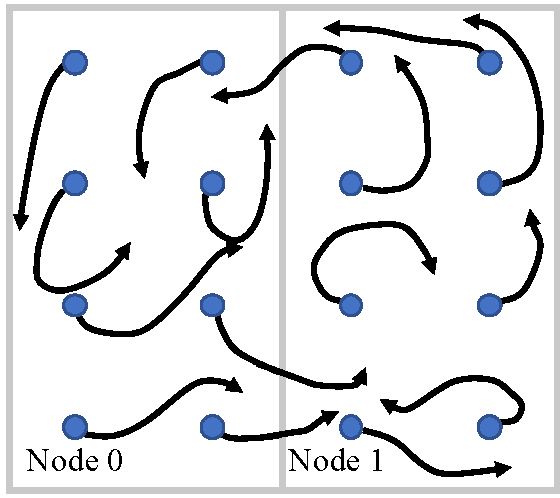
\includegraphics[width=\linewidth]{Images/notion_dist_1.pdf}
\caption{}
\label{fig:dist_1}
\end{subfigure}
\begin{subfigure}{0.16\textwidth}
\centering
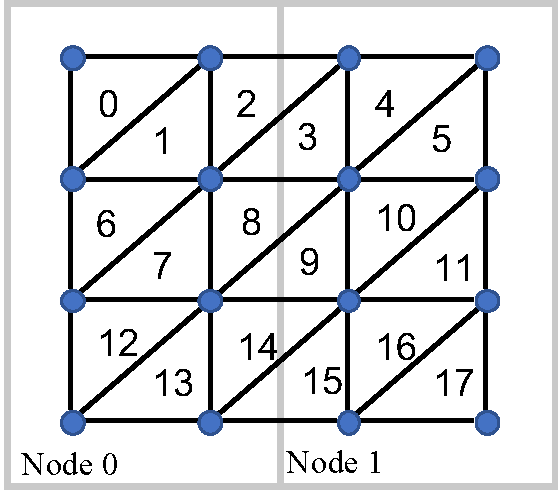
\includegraphics[width=\linewidth]{Images/notion_dist_2.pdf}
\caption{}
\label{fig:dist_2}
\end{subfigure}
\begin{subfigure}{0.16\textwidth}
\centering
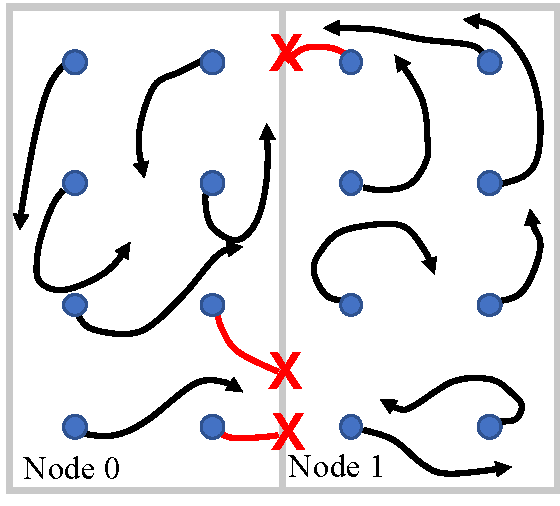
\includegraphics[width=\linewidth]{Images/notion_local_1.pdf}
\caption{}
\label{fig:local_1}
\end{subfigure}
\begin{subfigure}{0.16\textwidth}
\centering
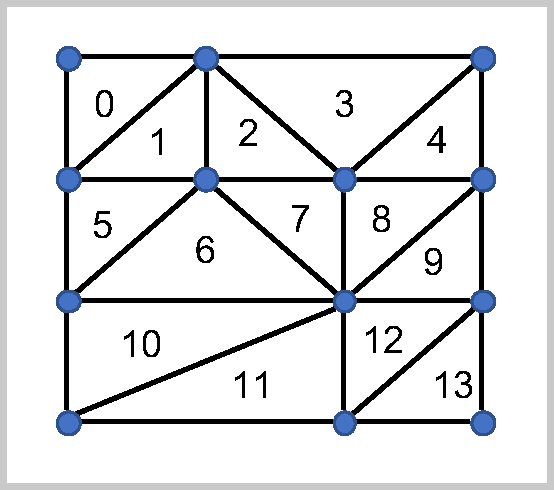
\includegraphics[width=\linewidth]{Images/notion_local_2.pdf}
\caption{}
\label{fig:local_2}
\end{subfigure}
\begin{subfigure}{0.35\textwidth}
\centering
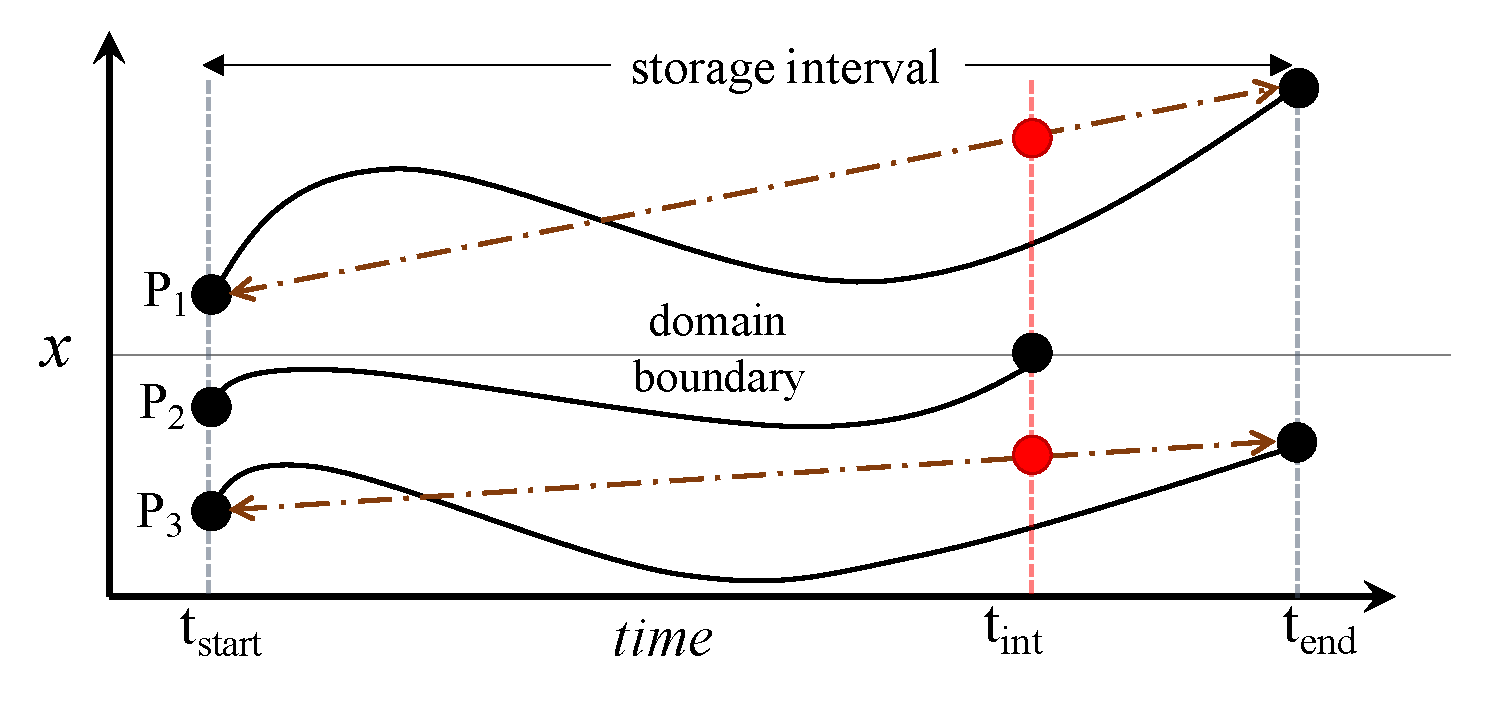
\includegraphics[width=\linewidth]{Images/early_termination.pdf}
\vspace{-7mm}
\caption{}
\label{fig:early_termination}
\end{subfigure}
\caption{Figures~\ref{fig:dist_1} and~\ref{fig:local_1} notionally illustrate the in situ computation of Lagrangian$_{Dist}$ and Lagrangian$_{Local}$ flow maps, respectively. Figures~\ref{fig:dist_2} and~\ref{fig:local_2} show the corresponding global triangulations. Figure~\ref{fig:early_termination} illustrates a case of early termination, and is described in Section~\ref{sec:local}.}
%\caption{The examples demonstrate in situ computation and post hoc use of Lagrangian$_{Dist}$~(\ref{fig:dist_1},~\ref{fig:dist_2}) and Lagrangian$_{Local}$(\ref{fig:local_1},~\ref{fig:local_2}) flow maps.}
\vspace{-5mm}
\label{fig:notional_examples}
\end{figure*}
